\documentclass[12pt]{article}

\usepackage[utf8]{inputenc}
\usepackage[T1]{fontenc}
\usepackage[spanish,es-noquoting]{babel}
\usepackage[letterpaper,margin=2.4cm]{geometry}
\usepackage{newtxtext}
\usepackage{graphicx}
\graphicspath{{../tesis/images/}}
\usepackage{caption}
\usepackage{xcolor}
\usepackage{mdframed}
\usepackage{titlesec}
\usepackage{enumitem}
\usepackage{float}
\usepackage[hidelinks]{hyperref}

\definecolor{azul}{HTML}{0B3D91}
\definecolor{rojo}{HTML}{C0392B}
\definecolor{gris}{HTML}{4A4A4A}
\definecolor{suave}{HTML}{F2F5F9}

\titleformat{\section}{\Large\bfseries\color{azul}}{}{0pt}{}
\titlespacing*{\section}{0pt}{20pt}{8pt}
\setlist{nosep, leftmargin=1.4em}
\captionsetup{font={small,it}, labelformat=empty}
\linespread{1.12}

\newmdenv[backgroundcolor=suave, linewidth=0pt, skipabove=10pt, skipbelow=12pt,
          innertopmargin=10pt, innerbottommargin=10pt,
          innerleftmargin=12pt, innerrightmargin=12pt]{idea}

\begin{document}

\thispagestyle{empty}
\begin{center}
{\Huge\bfseries ¿Qué hace esta tesis?}\\[4mm]
{\large\color{gris} Contar rocas en Marte sin mirar las fotos}\\[10mm]
{\normalsize Juan Pablo Delgado Castro}\\[1mm]
{\small\color{gris} Ciencia de Datos · Universidad Externado de Colombia}
\end{center}

\vspace{6mm}

\begin{idea}
\noindent\textbf{En una frase.} Existen unos mapas de Marte que alguien pintó a mano, y que
hasta ahora solo se usaban para enseñarle a una inteligencia artificial a reconocer el
terreno. Esta tesis los usa para otra cosa: \textbf{medir}. Y al medirlos, descubre que esos
mapas tienen un defecto que nadie había documentado.
\end{idea}

\section{El problema: las rocas estorban}

En Marte hay vehículos robot —los \textit{rovers}— que recorren la superficie. No se
conducen en directo: la señal tarda entre 3 y 22 minutos en llegar, así que cada movimiento
se planifica desde la Tierra con las fotos del día anterior.

En ese contexto, una roca no es un detalle del paisaje. Es un obstáculo que puede bloquear
el camino, obligar a un rodeo costoso o romper algo. Las ruedas del rover
\textit{Curiosity} se perforaron antes de tiempo por circular sobre roca con aristas
afiladas, y eso obligó a cambiar la forma de conducirlo.

Por eso interesa saber, de cada foto: \textbf{¿cuánta roca hay?} y \textbf{¿cuántas rocas
hay?}

\section{El material: un mapa pintado a mano}

Existe un proyecto de la NASA llamado \textbf{AI4Mars}. Miles de voluntarios de todo el
mundo se sentaron frente a fotos de Marte y las pintaron, como un libro para colorear: esto
es arena, esto es suelo, esto es roca. Píxel por píxel, en más de 16\,000 fotos.

El resultado es que cada foto tiene, al lado, un \textbf{mapa de colores} que dice qué hay
en cada punto.

\begin{figure}[H]
  \centering
  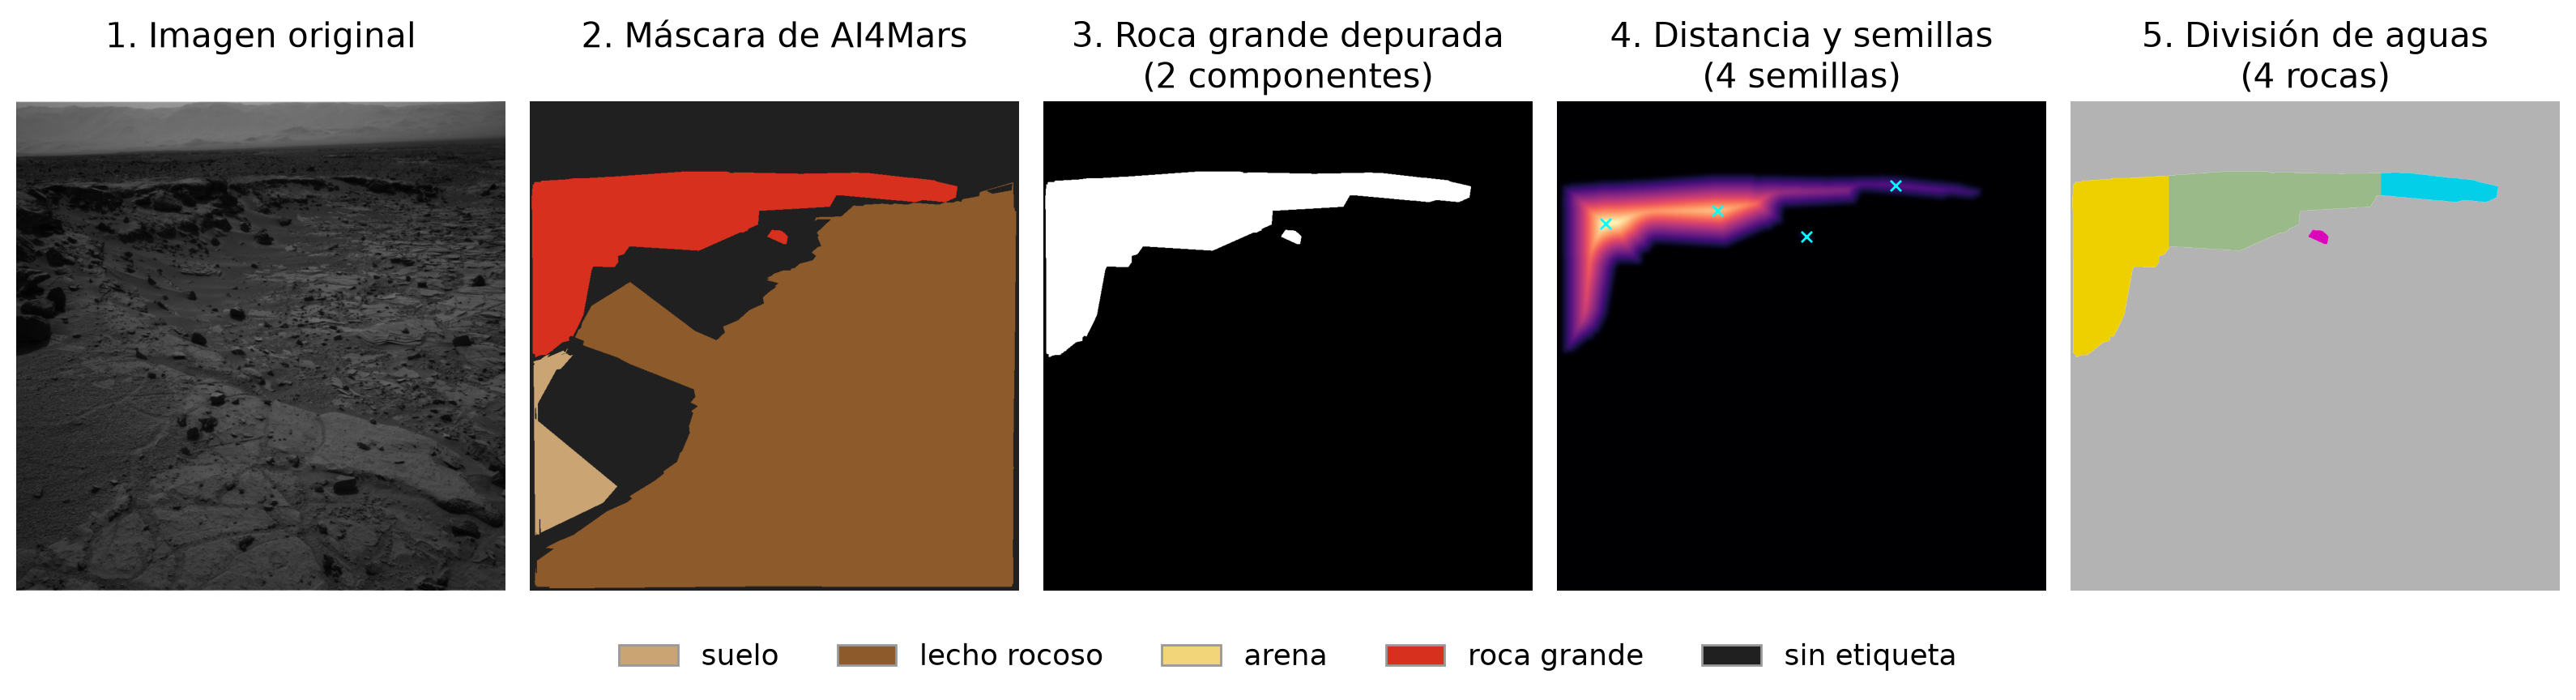
\includegraphics[width=0.86\textwidth]{Figura_11_procedimiento_paso_a_paso.png}
  \caption{A la izquierda, la foto real de Marte. A su lado, el mapa que pintaron los
    voluntarios. Los tres paneles restantes son los pasos del procedimiento de esta tesis.}
\end{figure}

\section{La idea de la tesis}

Hasta ahora, todo el mundo usaba esos mapas para lo mismo: \textbf{entrenar inteligencia
artificial}. El mapa hacía de «respuesta correcta» contra la que se corrige un programa
hasta que aprende a reconocer el terreno solo.

\begin{idea}
\noindent\textbf{La observación de partida.} Ese mapa no es solo la respuesta de un examen
para una máquina. \textbf{Es en sí mismo una medición.} Si un punto del mapa dice «aquí hay
roca», entonces contar puntos ya da una medida de cuánta roca hay — sin entrenar nada, sin
inteligencia artificial, y con una calculadora conceptualmente muy simple.
\end{idea}

Eso es lo que hace esta tesis: tomar 16\,064 mapas y convertirlos en números.

\section{Lo fácil y lo difícil}

\subsection*{Medir cuánta roca hay: fácil}

Es contar. Del total de puntos que alguien pintó, ¿qué porcentaje quedó pintado como roca?
Si de 45 puntos pintados 30 son roca, la respuesta es 67\,\%.

\subsection*{Contar cuántas rocas hay: difícil}

Aquí aparece el problema de verdad. El mapa dice \textit{dónde} hay roca, pero
\textbf{no dice dónde termina una roca y empieza otra}. Si dos rocas están pegadas, en el
mapa quedan como una sola mancha.

Hay que separarlas con geometría, y la idea es bonita:

\begin{enumerate}
  \item A cada punto de la mancha se le pregunta: \textit{¿a qué distancia estás del borde?}
  \item Los puntos del centro están lejos del borde; los del borde, cerca.
  \item Si imaginamos esa distancia como \textbf{altura}, la mancha se convierte en un
    paisaje: cada roca es una \textbf{colina}, y el punto donde dos rocas se tocan es un
    \textbf{valle}, porque ahí el borde está cerca por los dos lados.
  \item Se corta por el valle. Que es, exactamente, donde cualquiera de nosotros separaría
    las dos rocas a simple vista.
\end{enumerate}

\begin{idea}
\noindent\textbf{Y aquí está el problema que descubrió la tesis.} Ese método solo funciona
\textbf{si hay un valle}. Si el voluntario, en vez de pintar cada roca por separado, pintó
un manchón grande y liso encima de un montón de rocas, entonces no hay valles: hay una
meseta. Y el método devuelve \textbf{una sola roca}, por muchas que haya ahí dentro.
\end{idea}

\begin{figure}[H]
  \centering
  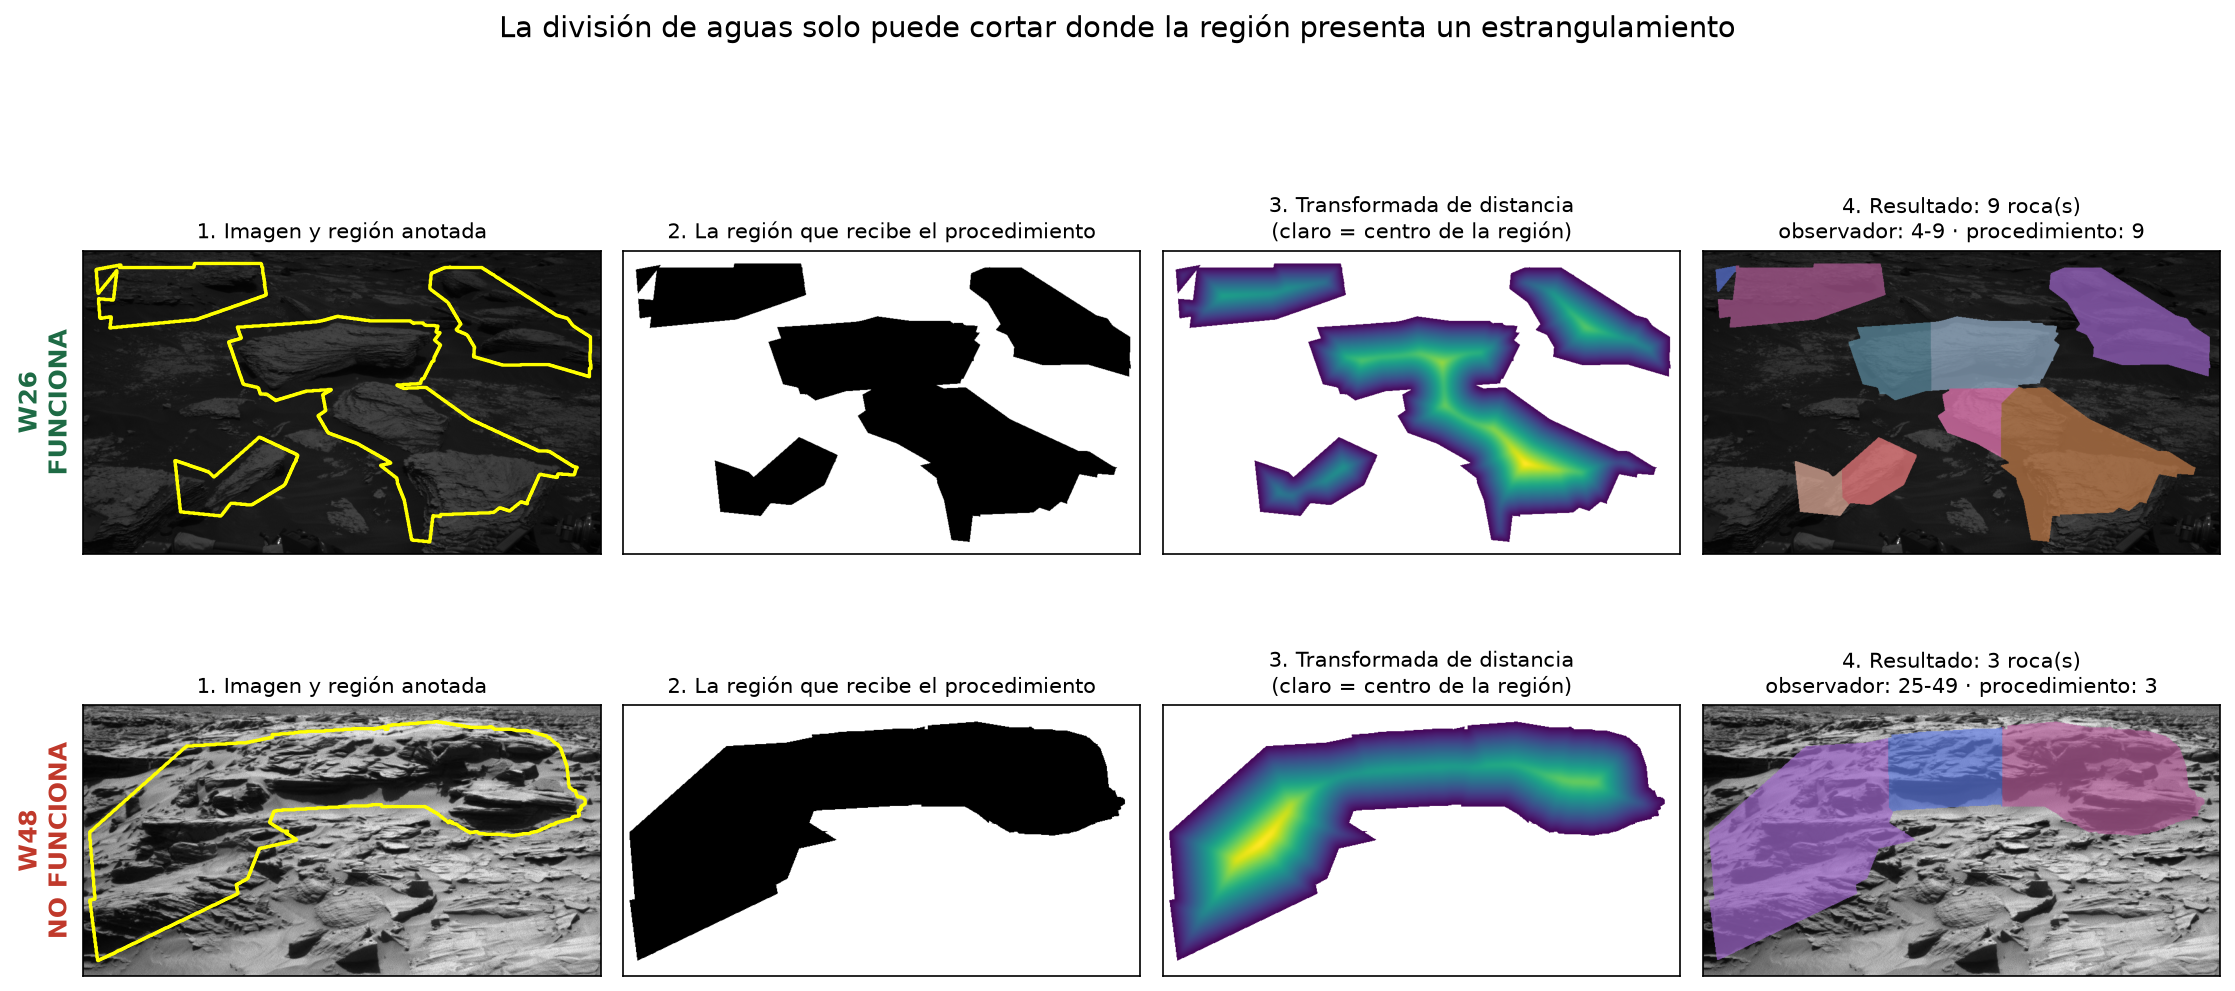
\includegraphics[width=\textwidth]{Figura_28_mecanismo_subconteo.png}
  \caption{Arriba funciona: el voluntario pintó cada bloque por separado, se ven los valles
    y el método cuenta 9 rocas. Abajo falla: un solo manchón sobre un campo entero de rocas,
    sin valles, y el método cuenta 3 donde una persona contó más de 25.}
\end{figure}

\section{Lo que se encontró}

\subsection*{1. Los mapas exageran cuánta roca hay}

Este es el hallazgo principal, y es un poco incómodo para el proyecto AI4Mars.

Piénsalo desde el lado del voluntario. La roca es fácil y satisfactoria de pintar: tiene
bordes claros, se distingue bien. El suelo y la arena son extensiones enormes y aburridas,
sin bordes. Así que mucha gente pintó la roca completa\dots{} y dejó buena parte del suelo
sin pintar.

Como el porcentaje se calcula sobre \textbf{lo que está pintado}, el suelo que falta
desaparece de la cuenta y la roca parece mucho más abundante de lo que es.

\begin{idea}
\noindent\textbf{Cómo se demostró.} El propio conjunto de datos incluye 322 mapas pintados
por \textbf{especialistas de la NASA}, que sí pintaron todo. Se les aplicó exactamente el
mismo programa, sin cambiar nada.

\smallskip
\noindent Con los mapas de voluntarios sale \textbf{96,8\,\%} de roca. Con los de
especialistas, \textbf{46,1\,\%}. \emph{Menos de la mitad.}

\smallskip
\noindent Y la prueba de que la explicación es la correcta: los especialistas no encontraron
más roca — encontraron \textbf{más suelo}. Pintaron un 69\,\% de suelo y arena frente al
50\,\% de los voluntarios.
\end{idea}

\subsection*{2. El problema no son las fotos}

La explicación obvia sería que hacen falta fotos mejores. No es eso, y la tesis lo demuestra
con esta imagen:

\begin{figure}[H]
  \centering
  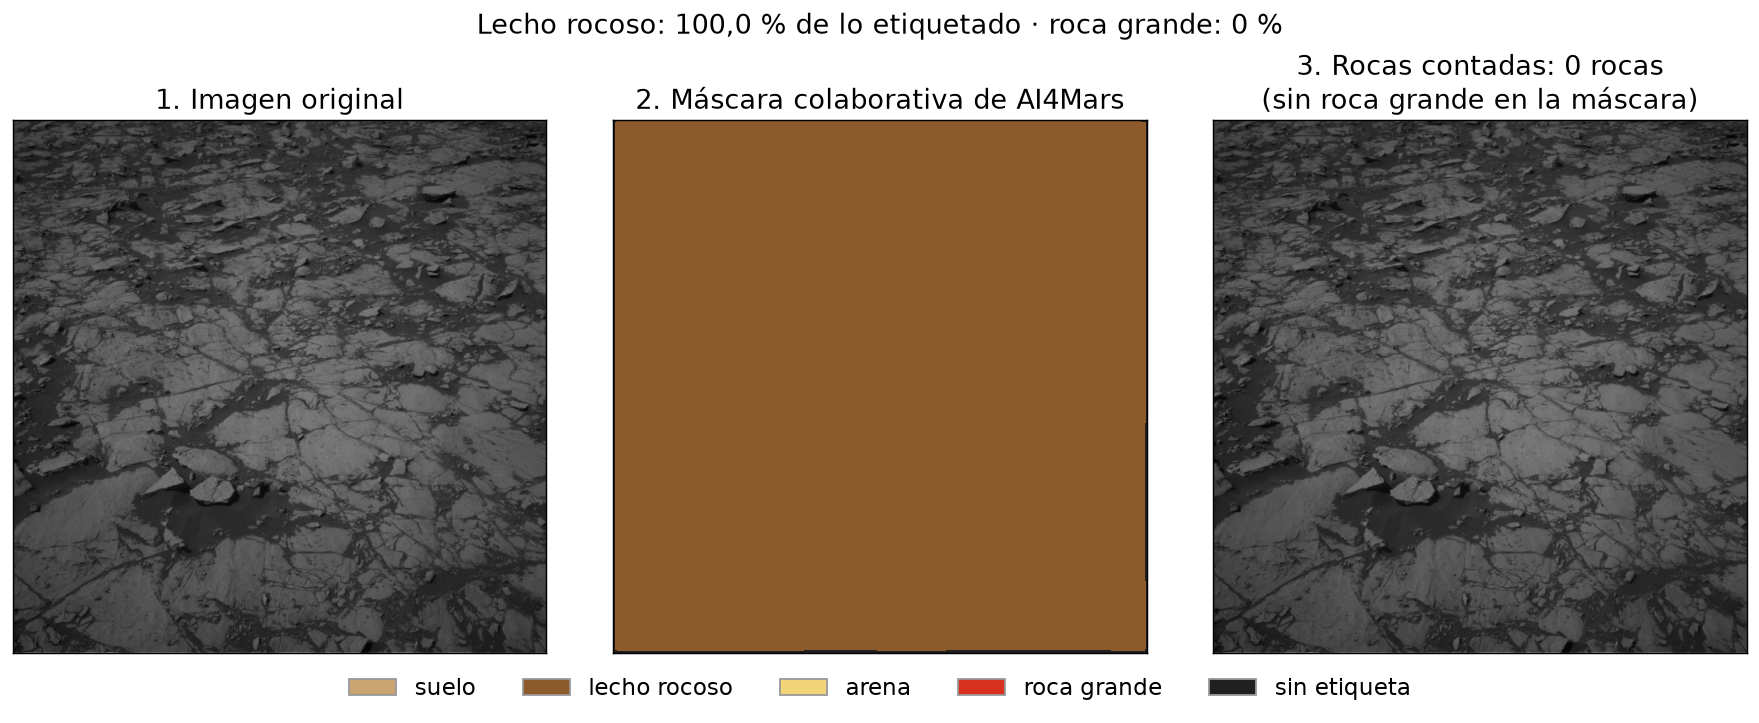
\includegraphics[width=\textwidth]{diag_bedrock_no_contado.png}
  \caption{Una foto llena de rocas perfectamente visibles. El voluntario la pintó entera
    como «un solo bloque de fondo». El programa cuenta cero rocas. La foto es excelente; lo
    que falla es la etiqueta.}
\end{figure}

\subsection*{3. Los mapas no marcan todas las rocas}

Esto se descubrió pidiéndole a una persona que contara rocas a mano en 60 fotos y comparando.
En 36 de esas 60, lo que el mapa marcó como «roca suelta» era \textbf{menos del 20\,\%} de
toda la roca de la foto.

Consecuencia importante y honesta: el número que produce la tesis \textbf{no es «cuántas
rocas hay en la foto»}. Es «cuántos bloques hay dentro de lo poco que el voluntario decidió
marcar». Pueden ser cosas muy distintas.

\section{¿Y para qué sirve todo esto?}

\subsection*{Lo que sí funciona}

La medida de \textbf{cuánta roca hay} funciona bien y se calculó para las 16\,064 fotos.
Sirve para comparar zonas y para ver cómo cambia el terreno a lo largo del recorrido del
rover.

Con esas medidas se construyó además un \textbf{sistema de avisos}: seis reglas que marcan
una foto cuando el terreno parece peligroso —demasiada arena, un bloque muy grande, muchas
rocas sueltas—. De las 16\,064 fotos, 104 salieron como riesgo alto.

\begin{figure}[H]
  \centering
  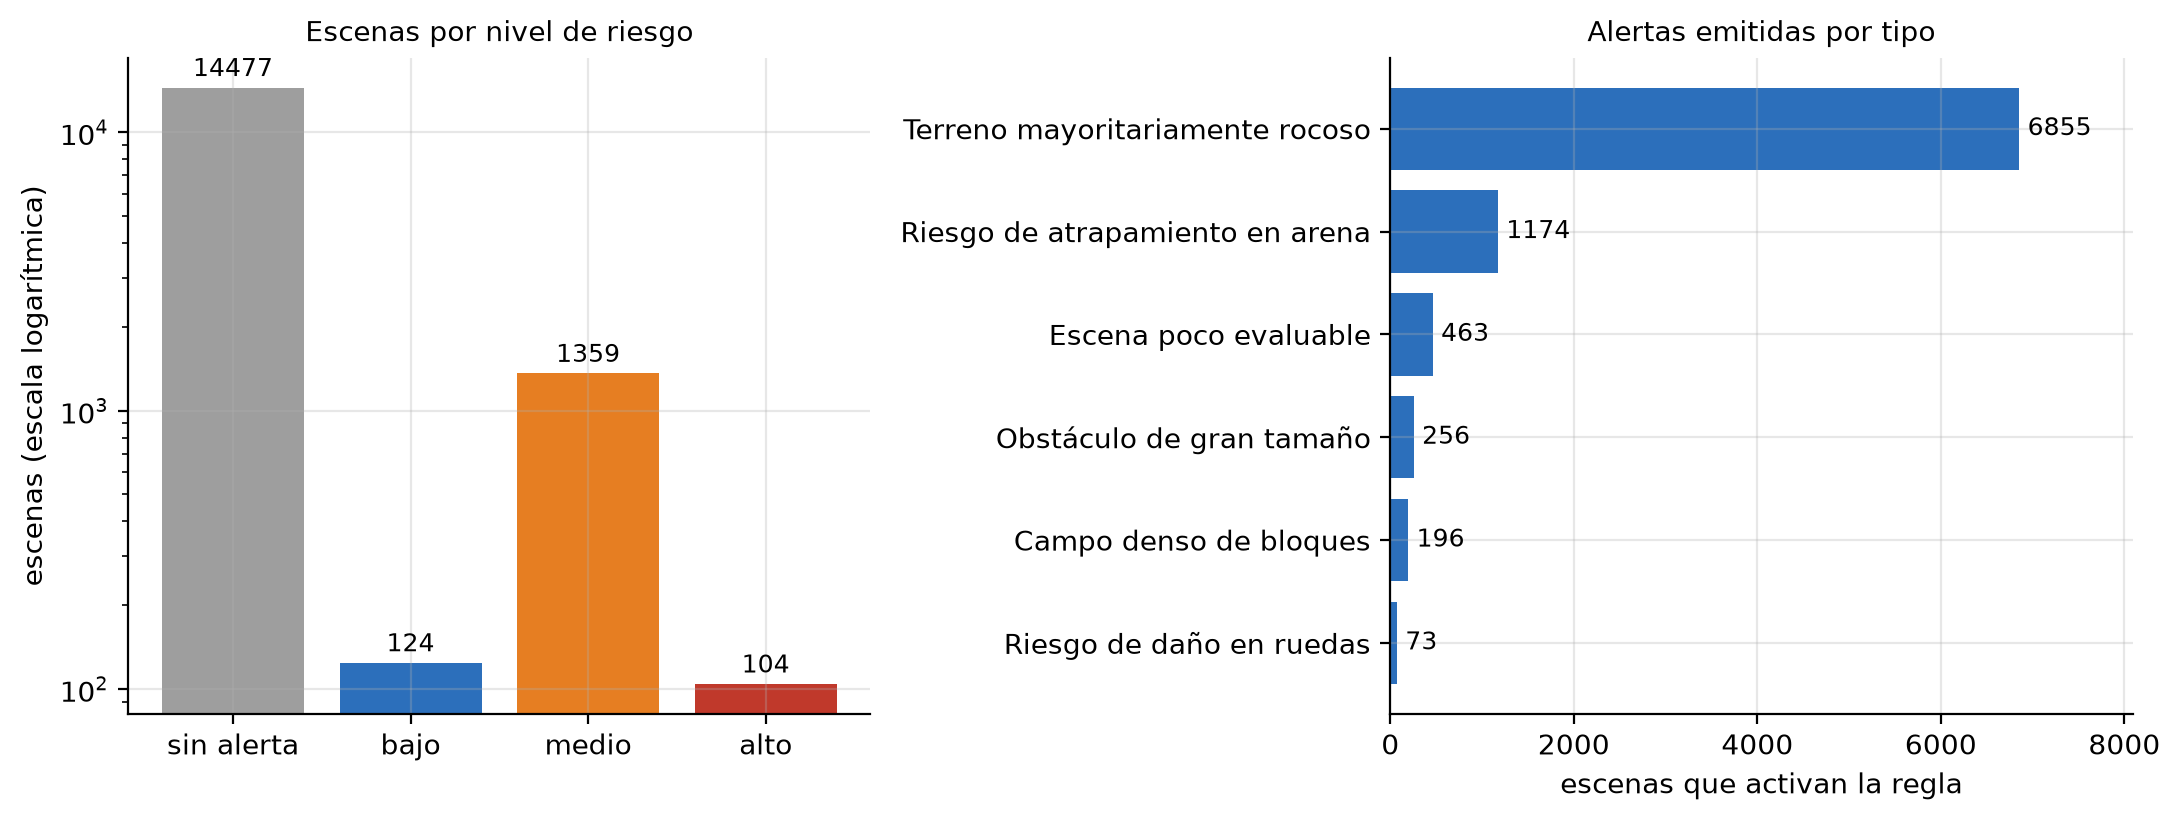
\includegraphics[width=\textwidth]{Figura_24_alertas_terreno.png}
  \caption{A la izquierda, cuántas fotos quedan en cada nivel de riesgo. A la derecha, qué
    tipo de aviso se activa con más frecuencia.}
\end{figure}

Y una \textbf{aplicación de escritorio} para consultar todo sin saber programar.

\subsection*{Lo que aporta a otros}

Este es el punto que hace la tesis útil más allá de sí misma.

Muchísimos trabajos de investigación usan estos mapas de AI4Mars como referencia: entrenan
un programa y luego miden qué tan bien lo hizo \textbf{comparándolo con estos mapas}. Si los
mapas exageran la roca, todas esas mediciones están comparando contra una referencia
torcida.

Nadie lo había medido. Esta tesis sí, y dice cuánto.

\section{Lo que esta tesis NO hace}

Por honestidad, y porque un trabajo serio declara sus límites:

\begin{itemize}\itemsep4pt
  \item \textbf{No mide cuánta roca hay en Marte.} Mide cuánta roca hay \textit{en estos
    mapas}, que exageran. Sirve para comparar entre fotos, no como dato absoluto.
  \item \textbf{No cuenta bien las rocas.} Se comparó con el conteo de una persona y no
    coincide. La tesis explica por qué y lo reporta como resultado, no lo esconde.
  \item \textbf{No mide en metros.} Los tamaños son relativos al encuadre de la foto: se
    sabe que una roca es grande o pequeña respecto a la escena, no cuántos centímetros mide.
  \item \textbf{No sirve para conducir el rover.} Necesita un mapa pintado a mano, y eso no
    existe en el momento en que las fotos llegan a la Tierra.
\end{itemize}

\begin{idea}
\noindent\textbf{Una última cosa, que suele sorprender.} Que el conteo no funcione no es un
fracaso de la tesis. La pregunta de investigación era \textit{cómo medir} estas cosas, y la
respuesta completa resultó ser: \textbf{una se puede medir y la otra no, y aquí está la
demostración de por qué no}. Saber dónde está el límite de un dato, y poder probarlo, es un
resultado — y le ahorra el camino a quien venga detrás.
\end{idea}

\vfill
\begin{center}
\small\color{gris}
El código, los datos y el documento completo están disponibles en\\
\url{https://github.com/NotJaayz/mars-agent-research}
\end{center}

\end{document}
